\documentclass[10pt,letterpaper]{memoir}
% memoir commands to define the text block geometry
\setulmarginsandblock{1in}{*}{*}
\setlrmarginsandblock{1in}{*}{*}

\usepackage{xparse}
\usepackage{blindtext}
\usepackage{enumitem}
\usepackage{graphicx}

\usepackage{amsmath,mathtools,amssymb}
% See https://texblog.net/latex-archive/maths/amsmath-matrix/ 
% for an explanation of this extention of the amsmath matrix commands.
% It's a way to enable "augmented matrices" using a new optional argument:
%
% \begin{pmatrix}[cc|c]
%     1 & 2 & 3\\
%     4 & 5 & 9
%   \end{pmatrix}
%
\makeatletter
\renewcommand*\env@matrix[1][*\c@MaxMatrixCols c]{%
  \hskip -\arraycolsep
  \let\@ifnextchar\new@ifnextchar
  \array{#1}}
\makeatother

\usepackage{bm} % bold math package

\usepackage{booktabs}
\usepackage{multirow}
\usepackage{hyperref}
\usepackage{systeme}

\usepackage{tcolorbox}
    \tcbuselibrary{skins}
    \tcbuselibrary{raster}
    \tcbuselibrary{skins}
\usepackage{tikz}
    \usetikzlibrary{arrows.meta}
\usepackage{tkz-base}
\usepackage{tkz-fct}    
\usepackage{pgfplots}
    \pgfplotsset{compat=newest}

% for inserting blanks that the students fill in
\usepackage{dashundergaps} % for \gap
\dashundergapssetup{
    teacher-mode=false, % set to true to show answers 
    gap-format=underline,
    teacher-gap-format=underline,
    gap-font={\ECFAugie\MTversion{augie}\color{black}},
    gap-numbers=false,
    gap-widen=true,
    gap-extend-percent=100, % note: making this too big might create errors
    gap-number-format=\,\textsuperscript{\normalfont(\thegapnumber)},
}

\usepackage{emerald}
\usepackage[subdued]{mathastext}% no italic for Augie anyhow
    \MTDeclareVersion[n]{lmvtt}{T1}{lmvtt}{m}{n}
    \MTfamily{augie}
    \Mathastext[augie]

\newcommand{\myHeadFootStyle}{\footnotesize\sffamily}
\copypagestyle{myPagestyle}{empty}
%
% FIXME
% The following header definitions do NOT work right in all cases.
% I have found that the chapter title sometimes gets picked up from
% a chapter that begins on the NEXT PAGE. Not sure what's going on.
% So I abandoned embedding the info in the header and instead updated
% \myLesson to print it out, and that seems to work find.
%
% \makeoddhead{myPagestyle}
%     {\,}
%     {\,}
%     {\myHeadFootStyle\chaptername\,\thechapter\,\,\myCurrentChapterTitle}
% \makeevenhead{myPagestyle} 
%     {\,}
%     {\,}
%     {\myHeadFootStyle\chaptername\,\thechapter\,\,\myCurrentChapterTitle}
\makeoddfoot{myPagestyle}
    {\myHeadFootStyle\myCurrentBookTitle}
    {\myHeadFootStyle\thepage}
    {\myHeadFootStyle\thechapter.\themyLessonCounter\,\,\myCurrentLessonTitle}
\makeevenfoot{myPagestyle}
    {\myHeadFootStyle\thechapter.\themyLessonCounter\,\,\myCurrentLessonTitle}
    {\myHeadFootStyle\thepage}
    {\myHeadFootStyle\myCurrentBookTitle}


\setlength{\parindent}{0em}
\setlength{\parskip}{0.75em}

\begin{document}
\pagestyle{plain}
\checkandfixthelayout
% \raggedbottom
\dashundergapssetup{teacher-mode=false,}

\newcommand{\myEmph}{\bfseries\itshape}
\newcommand{\myClassName}{{\tagged{pre-AP}{pre-AP }}Algebra 2}

% So I can save/restore \fboxsep
\newlength{\mySavedFboxsep}
\newcommand{\mySaveFboxsep}{\setlength{\mySavedFboxsep}{\fboxsep}}
\newcommand{\mySaveAndSetFboxsep}[1]{
    \setlength{\mySavedFboxsep}{\fboxsep}
    \setlength{\fboxsep}{#1}
}
\newcommand{\myRestoreFboxsep}{\setlength{\fboxsep}{\mySavedFboxsep}}

% A centered tcolorbox
%
% #1 - options to pass to tcolorbox
%
\NewDocumentEnvironment{myCenteredBox}{m}{%
    \begin{center}
    \begin{tcolorbox}[#1]
}{
    \end{tcolorbox}
    \end{center}
}


% A centered system of equations
%
\NewDocumentCommand{\myCenteredSysteme}{m}{%
    \begin{center}\systeme{#1}\end{center}
}

%
% This specialized command is my way of typesetting a table for
% students to use when solving systems of equations using matrices.
%
% - I make it really wide, because I need horizontal space. The increase in margin width 
%   is adjustable, but frankly, there are a lot of hard-coded dimensions in the table, so
%   I'm not positive that generality works well.
%
% - I put the content in a tikz picture with an OPAQUE background, since I 
%   plan to overlay this on top of Examples, which have dotted boxes around 
%   them at the "normal" margins.
%
% - The table uses the multirow package so that I can have the "Solution" box span two cells.
%
\NewDocumentCommand{\myWideMatrixTable}{O{-0.7in}}{
    \begin{adjustwidth}{#1}{#1}
        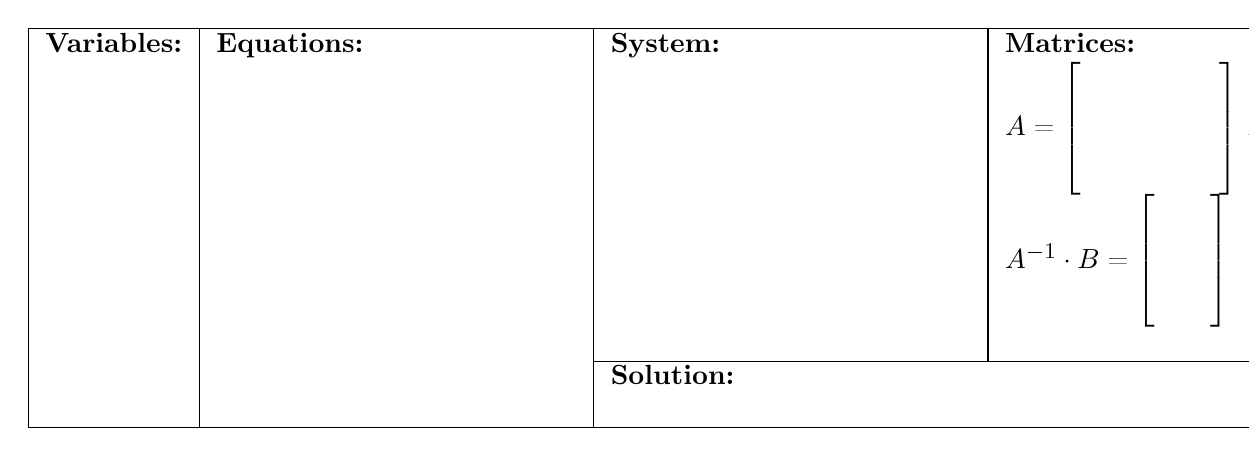
\begin{tikzpicture}
            \node
            [
                text width=1.25\textwidth, %I dinked with the multiplier to get balanced margins
                fill=white!30, 
                fill opacity=1,
                text opacity=1,
                inner sep=0pt,
            ]
            {%
                \begin{tabular}{|l|m{1.8in}|m{1.8in}|m{2.1in}|}
                    \hline
                    {\bfseries\scshape Variables:} & {\bfseries\scshape Equations:} & {\bfseries\scshape System:} & {\bfseries\scshape Matrices:} \\
                    % & & & \\
                    & & & 
                    \(
                        A = 
                        \begin{bmatrix}
                            \phantom{99} & \phantom{99} & \phantom{99} \\
                            \phantom{99} & \phantom{99} & \phantom{99} \\
                            \phantom{99} & \phantom{99} & \phantom{99} \\
                            \phantom{99} & \phantom{99} & \phantom{99} \\
                        \end{bmatrix}
                    \)
                    \(
                        B = 
                        \begin{bmatrix}
                            \phantom{999}\\
                            \phantom{999}\\
                            \phantom{999}\\
                            \phantom{999}\\
                    \end{bmatrix}
                    \)
                    \\
                    & & &
                    \(
                        A^{-1}\cdot B = 
                        \begin{bmatrix}
                            \phantom{9999}\\
                            \phantom{999}\\
                            \phantom{999}\\
                            \phantom{999}\\
                    \end{bmatrix}
                    \)
                    \\
                    & & & \\ \cline{3-4}
                    & & 
                    \multicolumn{2}{l|}{\bfseries\scshape Solution:}
                    \\ 
                    & & 
                    \multicolumn{2}{l|}{\,}
                    \\ 
                    \hline
                \end{tabular}
            };
        \end{tikzpicture}
    \end{adjustwidth}
}


{\small Pre-AP Algebra 2}\hfill Name: \rule{2in}{0.15mm}

{\bfseries\Large PAP HW 4.4 (DAY 2) A Sneak Peak at Linear Regression}\hfill Period: \rule{0.5in}{0.15mm}



\begin{tcolorbox}
    \itshape\small
    Work this problem if you have finished yesterday's sheet of problems.
    This is a ``warm up'' to the topic of 
    {\bfseries\itshape linear regression}, which we will discuss tomorrow.
\end{tcolorbox}




\section*{Four equations \& four unknown variables} 
Here are four $x$-$y$ points:
\begin{center}\begin{tabular}{cc}
    \toprule
    $x$ & $y$ \\
    \midrule
    -5 & 5 \\
    0 & -2 \\
    3 & 2 \\
    5 & 0 \\
    \bottomrule
\end{tabular}\end{center}
Using what you learned a few days ago,
find the equation of the cubic  
\[
    y = a + bx + cx^2 + dx^3
\]
that goes through
those four points.
Remember,
\begin{itemize}[itemsep=0in]
    \item You have four unknown variables, $a$, $b$, $c$, $d$.
    \item By evaluating the cubic at the four points, you get four equations
    involving the four unknow variables.
    \item Using the {\scshape Desmos Matrix Calculator}, 
    you can calculate $A^{-1}B$ to find the unknown variables.
\end{itemize}
(You'll probably need some scratch paper.)\vspace{1em}

\begin{minipage}{2in}
    {\Large
    $a$ = \gap{\hspace{1em}}\\[1em]
    $b$ = \gap{\hspace{1em}}\\
    }
\end{minipage}
\begin{minipage}{2in}
    {\Large
    $c$ = \gap{\hspace{1em}}\\[1em]
    $d$ = \gap{\hspace{1em}}\\
    }
\end{minipage}
\hrule





\section*{Graph it!}
Enter that function into the {\scshape Desmos Graphing Calculator}.
Does the curve seem to pass exactly through the four points in the table?

Answer yes or no: \gap{\hspace{3em}}

Does the point $(2,1)$ seem to be ``near'' the graph of the cubic function?

Answer yes or no: \gap{\hspace{3em}}\vspace{1em}
\hrule





\section*{Five equations \& four unknown variables?} 
So let's consider {\bfseries\itshape five} $x$-$y$ points.
\begin{center}\begin{tabular}{cc}
    \toprule
    $x$ & $y$ \\
    \midrule
    -5 & 5 \\
    0 & -2 \\
    3 & 2 \\
    5 & 0 \\
    2 & 1 \\
    \bottomrule
\end{tabular}\end{center}

Using all {\bfseries\itshape five} of those points,
formulate {\bfseries\itshape five} equations 
and write out the new $A$ and $B$ matrices below:
\par
{\Large
    \vspace{3em}
    \hfill $A = $\hspace{1.5in} \hfill $B = $\hspace{1.5in} \hfill
    \vspace{3em}
}

Use the {\scshape Desmos Graphing Calculator}
to calculate $A^{-1}B$. 
What happens? Explain what you think is going on.
\vspace{2.5in}
\hrule


\section*{Sneak peak at linear regression}

In a web browser (Safari, Chrome... on your phone), go to this URL:\\
\url{https://www.desmos.com/calculator/nzz8zxtguy}.

The graph there has a table of the same five data points that you used, above.
And it uses something called 
{\bfseries\itshape linear regression}
to find a cubic equation passing through those points.

This is something the $A^{-1}B$ matrix math was unable to do
(as you found above).

Linear regression uses more complicated matrix math 
to do this. 
So in fact it {\bfseries\itshape is} possible. 
It's just that the curve won't go through all five points exactly.
Linear regression is a method for finding the ``best'' curve that 
passes through all the points.
To see this, 
play with the slider on the graph. It changes the
$y$-coordinate of that fifth point. 

As you slide the slider,
you should be able to see that the curve no longer passes through 
all the points exactly.
Yet, it is possible to prove that the curve is the best one
in the sense of being {\itshape as close as possible to all the points
at the same time.}

We will talk more about linear regression tomorrow.
\end{document}
